\documentclass[11pt,a4paper]{article}
\usepackage[utf8]{inputenc}
\usepackage[T1]{fontenc}
\usepackage{lmodern}
\usepackage[french]{babel}
\usepackage[margin=2.1cm]{geometry}
\usepackage{microtype}
\usepackage{amsmath,amssymb}
\usepackage{booktabs}
\usepackage{array}
\usepackage[table]{xcolor}
\usepackage{graphicx}
\usepackage{caption}
\usepackage{eurosym}
\usepackage[most]{tcolorbox}
\definecolor{navy}{HTML}{1F3864}
\definecolor{bluemid}{HTML}{2E5496}
\definecolor{lightblue}{HTML}{D6E0F0}
\captionsetup{font=small,labelfont={bf,color=navy},labelsep=period}
\graphicspath{{../figures/}}
\newtcolorbox{cle}[1][]{colback=lightblue!40,colframe=navy,boxrule=0.6pt,
  arc=2pt,left=8pt,right=8pt,top=6pt,bottom=6pt,#1}

\title{\vspace{-1.2cm}\color{navy}\bfseries Le retour sur investissement de la conformité\\[2pt]
  \large Le capital libéré face au coût de remédiation}
\author{Kélian Kaddouri}
\date{27 juillet 2026}

\begin{document}
\maketitle
\vspace{-0.9cm}

\begin{cle}
\textbf{L'idée.} Chaque levier de conformité libère du capital (le $\Delta$SCR entre non
conforme et conforme, tableau de bord KPI) ; le remédier a un coût. On confronte les deux, et la
conformité cesse d'être un pur coût : c'est un levier de capital.
\end{cle}

\medskip
\begin{center}
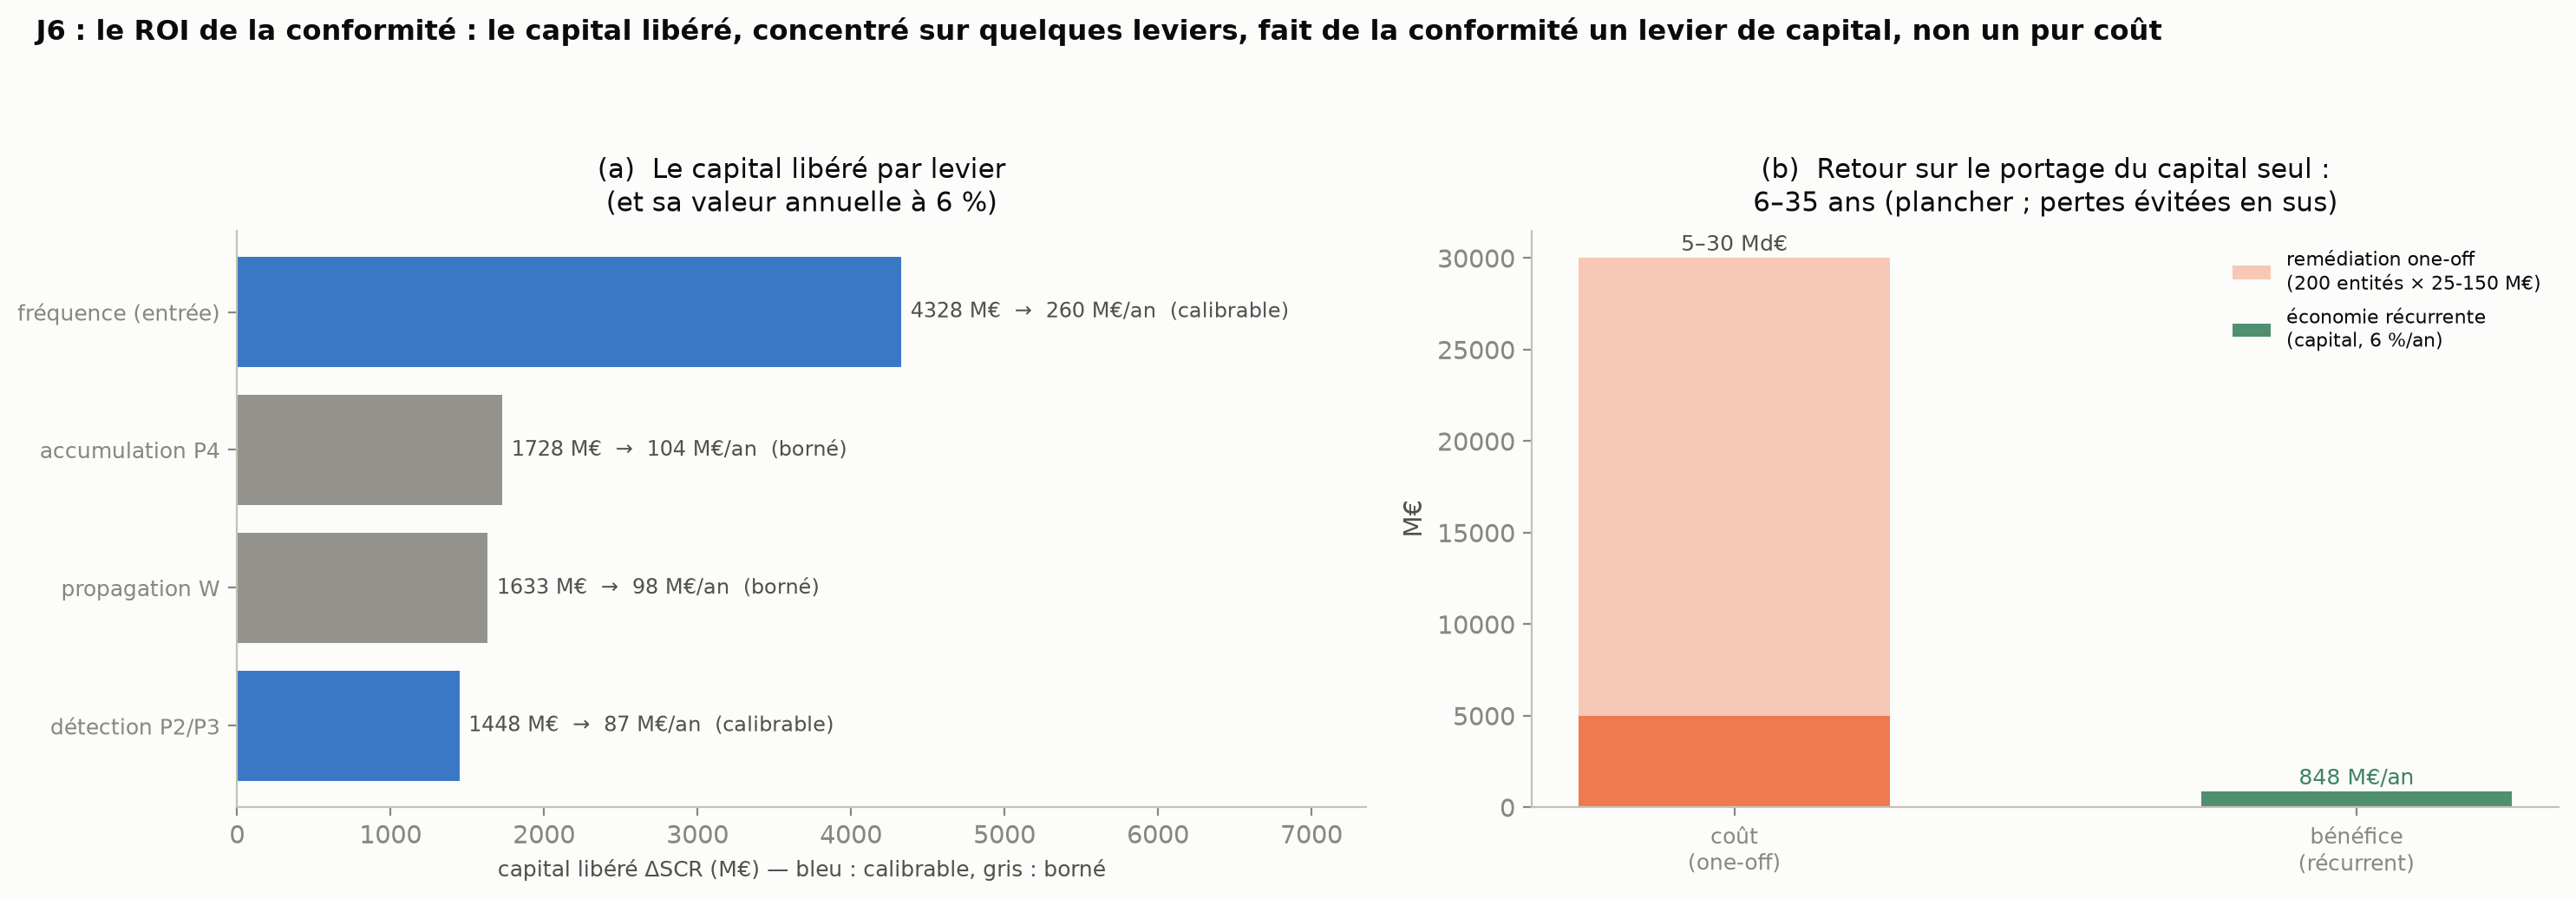
\includegraphics[width=\linewidth]{J6_roi_conformite.png}
\captionof{figure}{\textbf{(a)} le capital libéré par levier, classé, avec sa valeur annuelle à
$6\,\%$ (bleu : calibrable, gris : borné). \textbf{(b)} coût de remédiation \emph{one-off} contre
économie \emph{récurrente} de portage du capital.}
\end{center}

\noindent\textbf{Le capital libéré, valorisé.} Chaque levier libère $\Delta$SCR, dont la valeur
récurrente au coût du capital de Solvabilité~II (marge de risque, $6\,\%$) vaut
$6\,\%\times\Delta$SCR par an :
\begin{center}\small
\renewcommand{\arraystretch}{1.1}
\begin{tabular}{@{}l r r l@{}}
\toprule
\textbf{Levier} & \textbf{Capital libéré} & \textbf{Valeur/an} & \textbf{Statut} \\
\midrule
Fréquence (entrée)   & $4\,328$ M\euro & $260$ M\euro/an & calibrable \\
Accumulation P4      & $1\,728$ M\euro & $104$ M\euro/an & borné \\
Propagation $W$      & $1\,633$ M\euro & $98$ M\euro/an  & borné \\
Détection P2/P3      & $1\,448$ M\euro & $87$ M\euro/an  & calibrable \\
\bottomrule
\end{tabular}
\end{center}
La conformité totale libère $14\,139$ M\euro{} de SCR, soit $848$ M\euro/an, et ce capital est
\textbf{concentré} (la fréquence en porte près de la moitié). Face au coût de remédiation DORA
($\sim$25 à 150~M\euro{} par grande entité, estimations de place), le retour sur le \emph{seul}
portage du capital est de l'ordre de $6$ à $35$ ans --- un \textbf{plancher} conservateur, le
$\Delta$SCR étant surtout de la perte évitée ; les pertes évitées raccourcissent nettement ce
retour.

\begin{cle}[colback=orange!8,colframe=orange!70!black]
\textbf{Honnêteté et message.} Le bénéfice (capital libéré) est issu du modèle ; le coût est
externe et incertain, affiché comme tel. Mais la conclusion tient : \textbf{prioriser la
remédiation par capital libéré} --- les leviers \emph{calibrables} (fréquence, détection)
d'abord. On passe du score de criticité abstrait à un arbitrage économique chiffré, opposable à
une direction financière.
\end{cle}

\smallskip
\noindent\footnotesize\textcolor{navy}{\textbf{Source.}} Script
\texttt{9\_cas\_usage/50\_roi\_conformite.py}, figure \texttt{J6\_roi\_conformite.png}. Coût du
capital $6\,\%$ (marge de risque Solvabilité~II) ; coût DORA $\sim$25-150~M\euro/entité (conseil,
McKinsey 2025).

\end{document}
